\documentclass[12pt,a4paper]{article}
\usepackage[a4paper,top=1.5cm, bottom=1.5cm, left=1.5cm, right=1.5cm]{geometry}
\usepackage[T2A]{fontenc}
\usepackage[utf8]{inputenc}
\usepackage[russian]{babel}
\usepackage{amsmath}
\usepackage{amssymb}
\usepackage{graphicx}
\usepackage{floatrow}
\usepackage{booktabs}
\usepackage{wrapfig}
\usepackage{indentfirst}
\usepackage{lipsum}
\usepackage{subcaption}
\usepackage{float}
\usepackage{enumitem}
\restylefloat{table}

\newcommand{\figref}[1]{(см. рис. \ref{#1})}
\newcommand{\e}[1]{\text{$\cdot10^{#1}$}}

\title{Работа №77\\ Применения операционных усилителей}
\author{Симанкович Александр \\ Б01-104}
\date{\today}

\begin{document}
	\maketitle	
	
	\subsection*{1. Измерение коэффициента усиления ОУ}

	\begin{figure}[H]
		\centering
		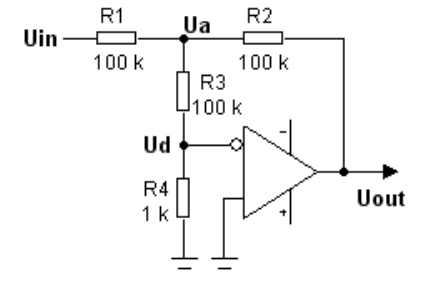
\includegraphics[width=0.5\linewidth]{res/1.png}
		\caption{Схема}
		\label{scheme1}
	\end{figure}

	Собираем схему с номиналами, указанными на рисунке $\ref{scheme1}$.
	
	Подаем на $U_{in}$ переменное напряжение с $f = 10$ Гц. Получаем $2U_{in} = 5.63$ В, $2U_a = 15$ мВ.
	
	Вычислим $A_0$:
	\begin{equation}
		A_0 = (1 + \frac{R_3}{R_4}) \cdot \frac{U_{out}}{U_a} = 3.5 \cdot 10^4.
		\label{ach1}
	\end{equation}
	
	\subsection*{2. Амплитудно-частотная характеристика ОУ}
	
	Пользуемся схемой $\ref{scheme1}$.
	
	Снимаем зависимость $A(f)$ согласно ($\ref{ach1}$).
	
	\begin{figure}[H]
		\centering
		\includegraphics[width=0.9\linewidth]{gen/2-afc.pdf}
		\caption{АЧХ ОУ}
		\label{ach2}
	\end{figure}
	
	Наклон графика составляет $a = -19.84$ дБ/декаду.

	По графику находим граничную частоту $f_{p0} = 1.42$ Гц и частоту единичного усиления $f_T = 1.44 \cdot 10^6$ Гц.
	
	\subsection*{3-4. Неинвертирующий и инвертирующие усилители}
	
	\begin{figure}[H]
		\centering
		\begin{minipage}[b]{.5\textwidth}
			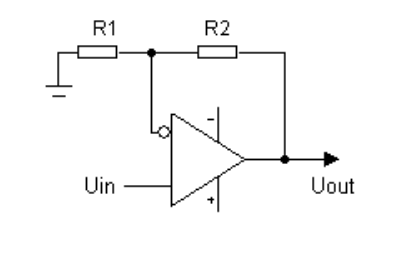
\includegraphics[width=0.9\linewidth]{res/3.png}
		\end{minipage}%
		\begin{minipage}[b]{.5\textwidth}
			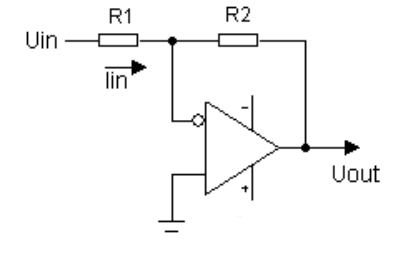
\includegraphics[width=0.9\linewidth]{res/4.png}
		\end{minipage}
		\caption*{Схемы неинвертирующего и инвертирующего усилителя}
	\end{figure}
	

	На схеме $R_1 = 1.10$ кОм, $R_2 = 94$ кОм.

	Измерим зависимость коэффициента усиления от частоты $K(f)$.

	\begin{figure}[H]
		\centering
		\includegraphics[width=0.9\linewidth]{gen/3-4-afc.pdf}
		\caption{АЧХ неинвертирующего и инвертирующего усилителей}
		\label{ach34}
	\end{figure}
	
	Для инвертирующего усилителя наблюдался сдвиг фаз на $\sim \pi$, что говорит об отрицательности коэффициента усиления.
	
	Граничные частоты почти совпадают, $F_p = 15.8$ кГц. Оценка $F_p = \beta f_T = 14.4$ кГц.
	Коэффициенты усиления $K = 100$.
	
	Также включим неинвертирующий усилитель по схеме повторителя ($R_1 = \infty, R_2 = 0)$.
	На частоте $f = 0.5$ МГц определим максимальную амплитуду неискаженного сигнала:
	$$ 2 U_{out}^{max} = 1.22 \; \text{В}.$$
	
	Оценка через максимальную скорость нарастания сигнала: $U_{mout} = \frac{V_{max}}{2 \pi f} = 0.95$ В.
	
	\begin{figure}[H]
		\centering
		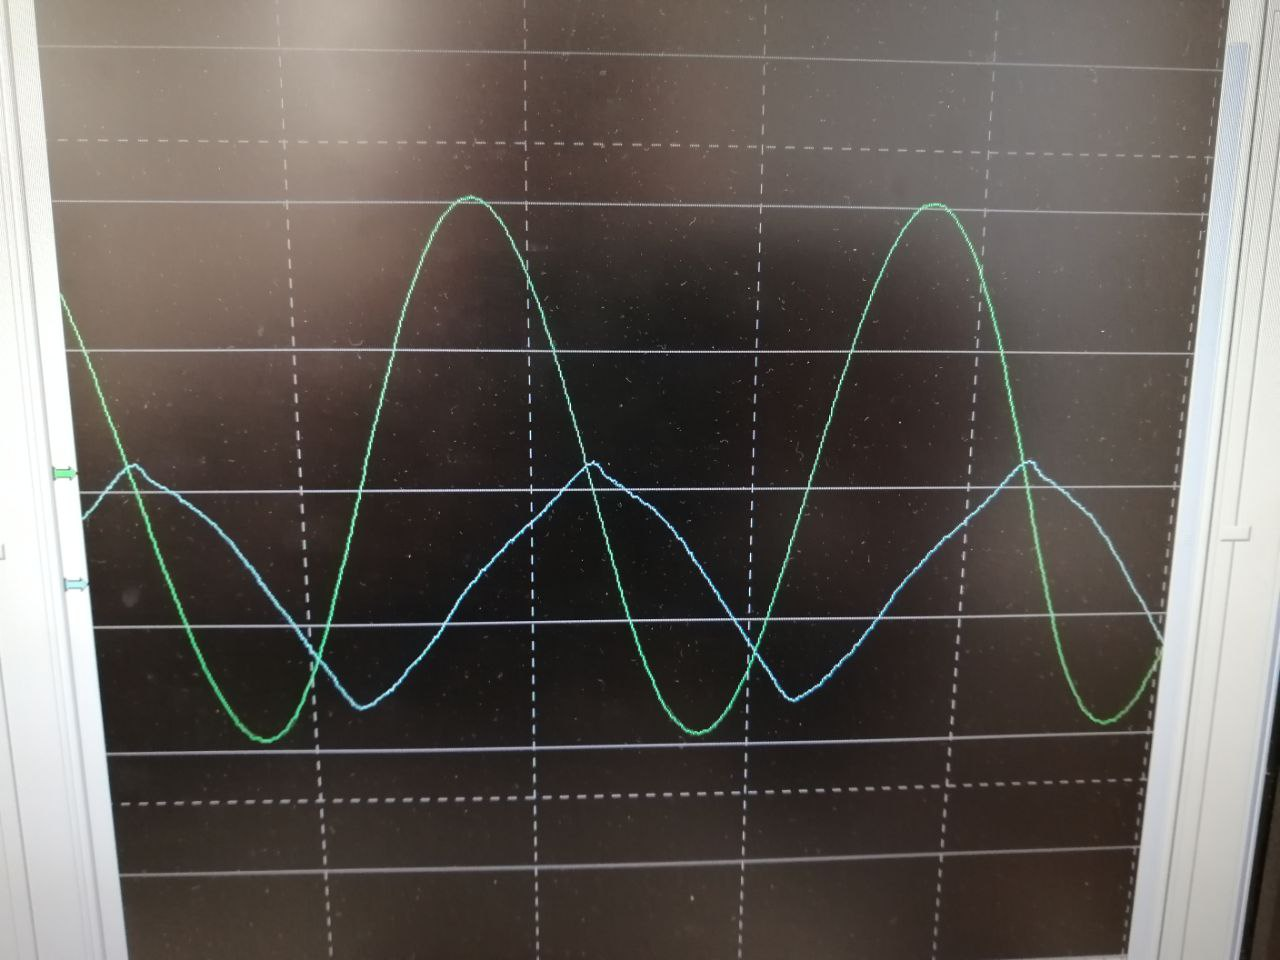
\includegraphics[width=0.5\linewidth]{res/repeat.jpg}
		\caption{Искаженный сигнал повторителя (1 кл. = 1 В)}
		\label{repeat}
	\end{figure}
	
	\subsection*{5. Разностный усилитель (вычитатель)}
	
	Соберем схему вычитателя:
	
	\begin{figure}[H]
		\centering
		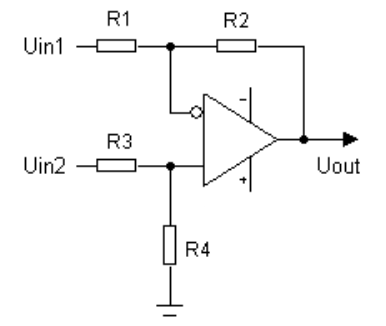
\includegraphics[width=0.5\linewidth]{res/5.png}
		\caption{Схема вычитателя}
		\label{subtract}
	\end{figure}
	
	Такая схема при $R_2 = R_4 = mR$, $R_1 = R_3 = R$ дает
	$$U_{out} = m (U_{in2} - U_{in1}).$$
	
	$R_2 = R_4 = 10 \; \text{кОм}$, $R_1 = R_3 = 2$ кОм. Таким образом, коэффициент вычитателя $m = R_2 / R_1 = 5$.
	
	Изучим коэффициент передачи вычитателя по обоим входам (парный вход закорачивается на землю):
	
	\begin{figure}[H]
		\centering
		\includegraphics[width=0.8\linewidth]{gen/5-single.pdf}
		\caption{АЧХ одиночных входов}
		\label{single}
	\end{figure}

	При подключении первого входа наблюдается сдвиг фаз на $\sim \pi$.
	По графику видно, что коэффициент усиления в полосе пропускания $K \approx m = 5$.
	
	Также проверим синфазный вход (оба входа подключены к одному потенциалу):
	$$U_{in} = 1 \; \text{В} \qquad U_{out} = 0.17 \; \text{В}. $$
	Как мы видим, $U_{out}$ мало.
	
\end{document}